\documentclass[slidestop]{beamer}
\usepackage[utf8]{inputenc}
\usepackage{pgf}
\usepackage{algorithmic}
\usepackage{wrapfig}
\usepackage{array}
\usepackage{subfigure}
\usepackage{xmpmulti}
\usepackage{listings}

\usetheme{JuanLesPins}
\usecolortheme{beaver}
\setbeamertemplate{navigation symbols}{}
\setbeamertemplate{footline}[frame number]
\title[B.A.T.M.A.N. V: what's coming next?]{B.A.T.M.A.N. V: what's coming next?}
\author{Marek Lindner \& Antonio Quartulli}
\date{May 14th, 2014\\WirelessBattleMeshv7 - Leipzig}
\institute[]{B.A.T.M.A.N.-Advanced\\www.open-mesh.org}

\newcommand{\cfbox}[2]{
	\colorlet{currentcolor}{.}
	{\color{#1}
	\fbox{\color{currentcolor}#2}}
}


\begin{document}

\begin{frame}
	\titlepage
\end{frame}

\section{Introduction}
\begin{frame}[c]
	\frametitle{A few words about batman-adv\dots}

	The B.A.T.M.A.N. protocol was initiated in Berlin, 2006. The first edition was developed as a daemon, and moved to kernel space in 2007 to improve performance.

	Characteristics:
	\begin{itemize}
		\item L2 routing (MAC address layer)
		\item runs on any Ethernet capable device (e.g. 802.3, 802.11, and 802.15.1)
		\item encapsulates incoming ether frames and handles all forwarding/delivery
		\item agnostic to IP or any L3 protocol
		\item supports non-mesh clients with gateway selection, roaming \& more
		\item part of the Linux kernel, thus shipped by default in most Linux distributions (modprobe batman-adv)
	\end{itemize}
\end{frame}

\begin{frame}[c]
	\frametitle{What we are NOT going to talk about today}
	\begin{itemize}
		\item backward compatibility (TVLV, compat number, etc)
		\item VLAN-ization of non-mesh client handling
		\item fragmentation v2.0 (we fragment everything!)
		\item extended AP isolation
		\item multicast improvements
		\item inter-connecting batman clouds
		\item layer2 anycast support
		\item DHT generalization (IPv6 address caching, ..)
		\item ...
	\end{itemize}
\end{frame}

\begin{frame}[c]
	\frametitle{Today's topics}
	\begin{itemize}
		\item B.A.T.M.A.N. V introduction
		\item network-wide multi-interface optimizations
		\item protocol overview (ELP/OGMv2)
		\item throughput based metric
		\item current status / practical tips
		\item next steps
	\end{itemize}
\end{frame}

\section{Multi-if routing}
\begin{frame}[c]
	\frametitle{Network-wide multi-interface optimization}

	brief recap:

	\begin{itemize}
		\item batman-adv supports link-local multi-iface optimizations since early 2010
		\item results were good but we can do better ..
	\end{itemize}

	\addvspace{1.0cm}

	B.A.T.M.A.N. V roadmap (extract):

	\begin{itemize}
		\item differentiation between half duplex / full duplex
		\item take advantage of the many interfaces devices are powered with today
		\item maximizing traffic throughput applying rules to the traffic flow
	\end{itemize}
\end{frame}

\begin{frame}[c]
	\frametitle{Network-wide multi-interface optimization (2)}

	in a nutshell:
	\begin{figure}
		\centering
		\includegraphics[scale=0.4]{images/multi-if1.pdf}
	\end{figure}
\end{frame}

\begin{frame}[c]
	\frametitle{Network-wide multi-interface optimization (3)}

	\begin{figure}
		\centering
		\includegraphics[scale=0.4]{images/multi-if2.pdf}
	\end{figure}
\end{frame}

\begin{frame}[c,fragile]
	\frametitle{Network-wide multi-interface optimization (4)}

	The tables:

	\begin{itemize}
		\item each interface has its own routing table
		\item the default table is used for traffic originating from the host itself
	\end{itemize}

	\begin{lstlisting}[basicstyle=\tiny]
# batctl o
[B.A.T.M.A.N. adv master-b82b9b2, MainIF/MAC: wlan0/node2_wlan0 (bat0 BATMAN_IV)]
 Originator last-seen (#/255)     Nexthop [outIF]:   Potential nexthops ...
 node3_wlan0   0.670s   (255) node3_wlan0 [wlan0]: node3_wlan1 (255) node3_wlan0 (255)
 node1_wlan0   0.920s   (255) node1_wlan1 [wlan1]: node1_wlan1 (255) node1_wlan0 (254)

# batctl o -i wlan0
[B.A.T.M.A.N. adv master-b82b9b2, IF/MAC: wlan0/node2_wlan0 (bat0 BATMAN_IV)]
 Originator last-seen (#/255)     Nexthop [outIF]:   Potential nexthops ...
 node3_wlan0   0.560s   (252) node3_wlan1 [wlan1]: node3_wlan1 (252) node3_wlan0 (240)
 node1_wlan0   0.850s   (255) node1_wlan1 [wlan1]: node1_wlan1 (255) node1_wlan0 (238)

# batctl o -i wlan1
[B.A.T.M.A.N. adv master-b82b9b2, IF/MAC: wlan1/node2_wlan1 (bat0 BATMAN_IV)]
 Originator last-seen (#/255)     Nexthop [outIF]:   Potential nexthops ...
 node3_wlan0   0.260s   (253) node3_wlan0 [wlan0]: node3_wlan1 (240) node3_wlan0 (253)
 node1_wlan0   0.510s   (255) node1_wlan0 [wlan0]: node1_wlan1 (240) node1_wlan0 (255)
	\end{lstlisting}

\end{frame}

\begin{frame}[c]
	\frametitle{Network-wide multi-interface optimization (5)}

	The benefits:
	\begin{figure}
		\centering
		\includegraphics[scale=0.175]{images/alternating-limited-view.pdf}
	\end{figure}
\end{frame}


\begin{frame}[c]
	\frametitle{Network-wide multi-interface optimization (6)}

	\begin{figure}
		\centering
		\includegraphics[scale=0.3]{images/net-wide-multiif.pdf}
	\end{figure}
\end{frame}

\section{Routing protocol}
\begin{frame}[c]
	\frametitle{protocol overview}
	\begin{itemize}
		\item evolution instead of revolution
		\item design goals
			\begin{itemize}
				\item simplification
				\item gain flexibility to better support diverse scenarios
				\item reduce overhead
			\end{itemize}
	\end{itemize}
\end{frame}

\begin{frame}[c]
	\frametitle{protocol overview - ELP}
	\begin{figure}
		\centering
		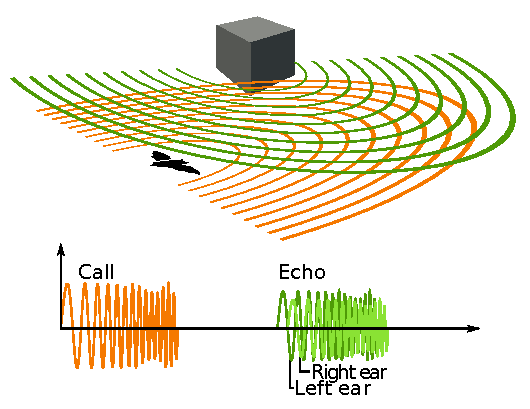
\includegraphics[scale=0.5]{ext_images/Animal_echolocation.pdf}
	\end{figure}

	ELP - Echo Location Protocol
	\begin{itemize}
		\item link sensing \& neighbour discovery
		\item no rebroadcast or forward of any kind
		\item short broadcast intervals
	\end{itemize}
\end{frame}

\begin{frame}[c]
	\frametitle{protocol overview - OGMv2}

	OGMv2 - Originator Message Protocol v2
	\begin{itemize}
		\item propagating routes in the mesh
		\item rebroadcast with stricter rules, yet simplified
		\item long broadcast intervals
	\end{itemize}

	\begin{figure}
		\centering
		\includegraphics[scale=0.2]{images/ogm-elp.pdf}
	\end{figure}
\end{frame}

\section{Metric}
\begin{frame}[c]
	\frametitle{A new metric}
	\begin{center}
		The dream of \textbf{throughput based routing}\dots
	\end{center}
\end{frame}

\begin{frame}[c]
	\frametitle{Reading throughput in kernel space (WiFi)}
	\textbf{Wireless links:} query the Rate Control algorithm
	\vfill
	\begin{figure}
		\centering
		\includegraphics[scale=0.3]{images/wireless-stack.pdf}
	\end{figure}
\end{frame}

\begin{frame}[c,fragile]
	\frametitle{Reading throughput in kernel space (WiFi) (2)}
	Our work focusses on \textbf{MinstrelHT}\\[0.5cm]
	\begin{lstlisting}[basicstyle=tiny]
	rate table
	\end{lstlisting}
\end{frame}

\begin{frame}[c]
	\frametitle{Throughput in kernel space (3)}
	\begin{center}
	\textbf{Wired links} (common scenario):\\
	read negotiated speed from the driver\\[0.5cm]
	\pause
	not the best approach, but it's easy\\[0.3cm]
	Example:
	\begin{figure}
		\centering
		\includegraphics[scale=0.25]{images/ethernet-switch.pdf}
	\end{figure}
	\end{center}
\end{frame}

\begin{frame}
	\frametitle{Throughput in kernel space (4)}
	But what about:
	\begin{itemize}
	\item VPN links
	\item tunnels
	\item \dots
	\end{itemize}
	manual configuration? what else?
\end{frame}

\begin{frame}[c,fragile]
	\frametitle{Throughput meter in batman-adv}
	\begin{itemize}
		\item started as Google Summer of Code project in 2012
		\item re-implementation of TCP on batman-adv
		\item no need for IPs (uses batman-adv identifiers)
		\item can also be used from userspace (using batctl)
		\item measures the ''payload`` throughput (no packet overhead)
	\end{itemize}
	\addvspace{0.5cm}
	Example:\\
	\begin{lstlisting}[basicstyle=\scriptsize]
	root@NodeA:~# batctl tm -t 3000 NodeB
	Throughput meter called towards NodeB
	Test duration 3010ms.
	Sent 20247000 Bytes.
	Throughput: 6.41 MB/s (53.81 Mbps)
	\end{lstlisting}
\end{frame}

\begin{frame}[c]
	\frametitle{Open problems}
	\begin{itemize}
		\item different RC algorithms (batman-adv is not aware!)
		\begin{itemize}
			\item different API implementation
			\item need for a different probing schema
		\end{itemize}
		\item different throughput from different link types
		\item real world testing
	\end{itemize}
\end{frame}

\section{Conclusions}
\begin{frame}[c]
	\frametitle{Current status}
	\begin{itemize}
		\item \textbf{cfg/mac80211 patches} under review by linux-wireless people
			and close to integration
		\item a working \textbf{B.A.T.M.A.N. V prototype} is available in our git
			repository (ordex/batman\_v branch)
		\item a working \textbf{throughput meter} protorype is available
			in our git reporitory (ordex/bw\_meter branch)
	\end{itemize}
\end{frame}

\begin{frame}[c,fragile]
	\frametitle{How to use B.A.T.M.A.N. V on my node}
	The batman-adv kernel module is already able to host more than one
	routing algorithm
	\begin{lstlisting}[basicstyle=\scriptsize]
	# cat /sys/kernel/debug/batman_adv/routing_algos
	BATMAN_IV
	BATMAN_V (only if compiled into the module)
	\end{lstlisting}
	\pause
	Benefits:
	\begin{itemize}
		\item the routing algorithm can be changed at runtime
	\end{itemize}
	\begin{lstlisting}[basicstyle=\scriptsize]
	# echo BATMAN_V >/sys/module/batman_adv/parameters/routing_algo
	# batctl if add -m bat0 wlan0
	\end{lstlisting}
	\pause
	\begin{itemize}
		\item both algorithms can be used at the same time (on two
			different interfaces)
	\end{itemize}
	\begin{lstlisting}[basicstyle=\scriptsize]
	# echo BATMAN_IV >/sys/module/batman_adv/parameters/routing_algo
	# batctl if add -m bat1 wlan1
	\end{lstlisting}
\end{frame}

\begin{frame}[c]
	\frametitle{How to use B.A.T.M.A.N. V on my node (2)}
	\begin{figure}
		\centering
		\includegraphics[scale=0.28]{images/multi-protocols.pdf}
	\end{figure}
\end{frame}

\begin{frame}[c]
	\begin{figure}
		\centering
		
\includegraphics[scale=0.28]{ext_images/batlogo_transparent.pdf}
	\end{figure}
	\begin{center}
	\Large{\textbf{Thank you for your attention\\[1cm]
	Questions?}}
	\end{center}
\end{frame}

\end{document}
